%
% chapter.tex -- Kapitel zur Funktionentheorie
%
% (c) 2021 Prof Dr Andreas Müller, Hochschule Rapperswil
%
% !TeX spellcheck = de_CH
\chapter{Funktionentheorie
\label{buch:chapter:funktionentheorie}}
\lhead{Funktionentheorie}
\rhead{}
Jede stetige reelle Funktion $f\colon I\to\mathbb{R}$ auf einem
Intervall kann beliebig genau durch Polynome, also durch
differenzierbare approximiert werden.
Für komplex differenzierbare Funktionen sieht die Situation
völlig anders aus.
Bereits die Funktion $z\mapsto \overline{z}$ kann in einer offenen
Teilmenge von $\mathbb{C}$ nicht durch Polynome in der Variablen $z$
approximiert werden.
Es stellt sich heraus, dass komplex differenzierbare Funktionen
immer eine konvergente Taylor-Reihe besitzen.
In Abschnitt~\ref{buch:funktionentheorie:section:analytisch} wird
ein Beispiel einer beliebig oft stetig differenzierbaren rellen
Funktion angegeben, die nur in $0$ verschwindet, deren Taylor-Reihe
in $0$ die Nullfunktion ist.

Wenn man also weiss, dass die Lösung eines Problems nicht nur eine
relle Funktion ist, sondern eine komplex differenzierbare Funktion,
dann unterliegt diese sehr viel strengeren Einschränkungen.
Mit der zugehörigen Potenzreihe können Funktionswerte leicht berechnet
werden, mit dem Cauchy-Integral können Singularitäten studiert werden
und mit der analytischen Fortsetzung kann man Lösungen über Singularitäten
auf der rellen Achse hinaus fortsetzen.

%
% holomorph.tex
%
% (c) 2021 Prof Dr Andreas Müller, OST Ostschweizer Fachhochschule
%
\section{Holomorphe Funktionen
\label{buch:funktionentheorie:section:holomorph}}
\rhead{Holomorphe Funktionen}

Wir betrachten in diesem Kapitel komplexwertige Funktionen,
\index{komplexwertige Funktion}%
die ein einem Teilgebiet der komplexen Ebene definiert sind.
Ein {\em Gebiet} ist eine offene Teilmenge $\Omega\subset \mathbb C$.
\index{Gebiet}%
{\em Offen} heisst, dass mit jedem Punkt $z_0\in\Omega$ eine Umgebung
\index{offen}%
\index{Umgebung}%
\[
U=\{z\in\mathbb Z\,|\,|z-z_0|<\varepsilon\}
\]
ebenfalls in $\Omega$ enthalten ist, also $U\subset \Omega$ für genügen
kleines $\varepsilon$.
Sei also $f(z)$ eine in $\Omega\subset\mathbb C$ definierte
Funktion $f\colon\Omega\to\mathbb C$.

Eine komplexwertige Funktion $f(z)$ kann betrachtet werden als zwei
reellwertige Funktionen von zwei Variablen $x$ und $y$:
\[
f(z)=\operatorname{Re}f(x+iy) + i \operatorname{Im}f(x+iy).
\]
Schreibt man
$\operatorname{Re}f(x+iy)=u(x,y)$
und
$\operatorname{In}f(x+iy)=v(x,y)$,
dann ist die komplexe Funktion vollständig durch reelle Funktionen
beschrieben.
Und natürlich wissen wir auch, was unter den Ableitungen der Funktionen
$u(x,y)$ und $v(x,y)$ zu verstehen ist.
Der Funktion $f(z)$ entspricht eine Abbildung $\mathbb R^2\to\mathbb R^2$
\index{Abbildung}%
\[
(x,y)\mapsto\begin{pmatrix}u(x,y)\\v(x,y)\end{pmatrix}.
\]
Die Ableitung einer solchen Funktion im Punkt $(x_0,y_0)$
ist eine lineare Abbildung von Vektoren, die in linearer Näherung
\index{lineare Naherung@lineare Näherung}
\index{Naherung@Näherung, lineare}
den Funktionswert bei $f(z_0 + \Delta z)$
\[
\begin{pmatrix}
u(x+\Delta x, y +\Delta y)\\
v(x+\Delta x, y +\Delta y)
\end{pmatrix}
=
\begin{pmatrix}
\frac{\partial u}{\partial x}&\frac{\partial u}{\partial y}\\
\frac{\partial v}{\partial x}&\frac{\partial v}{\partial y}
\end{pmatrix}
\begin{pmatrix} \Delta x\\\Delta y \end{pmatrix}
+o(\Delta x, \Delta y).
\]
In dieser Sicht einer komplexen Funktion gibt es keine einzelne Zahl, die
die Funktion einer Ableitung übernehmen könnte, die Ableitung
ist eine $2\times 2$-Matrix.

%
% Definition der komplexen Ableitungen
%
\subsection{Komplexe Ableitung}
Die Ableitung einer Funktion einer reellen Variablen wird mit Hilfe des
Grenzwertes
\[
f'(x_0)=\lim_{x\to x_0}\frac{f(x)-f(x_0)}{x-x_0}
\]
definiert, oder als diejenige Zahl $f'(x_0)\in\mathbb R$ mit der Eigenschaft,
dass
\begin{equation}
f(x)=f(x_0)+f'(x_0)(x-x_0) + o(x-x_0)
\label{komplex:abldef}
\end{equation}
gilt.
Der Term $x-x_0$ und die Gleichung \eqref{komplex:abldef} sind aber auch
für komplexe Argument sinnvoll, wir definieren daher

\begin{definition}
\label{buch:funktionentheorie:definition:differenzierbar}
Die komplexe Funktion $f(z)$ heisst im Punkt $z_0$ komplex differenzierbar
und hat die komplexe Ableitung $f'(z_0)\in\mathbb C$, wenn
\index{komplex differenzierbar}%
\index{komplexe Ableitung}%
\index{Ableitung!komplexe}%
\begin{equation}
f(z)=f(z_0) + f'(z_0)(z-z_0) +o(z-z_0)
\label{komplex:defkomplabl}
\end{equation}
gilt.
\end{definition}

\begin{beispiel}
Die Funktion $z\mapsto f(z)=z^n$ ist überall komplex differenzierbar
und hat die Ableitung $nz^{n-1}$.
Um dies nachzuprüfen, müssen wir die Bedingung~\eqref{komplex:defkomplabl}
verifizieren.
Aus einer wohlbekannten Faktorisierung von $z^n - z_0^n$ können wir den
Differenzenquotienten finden:
\begin{align*}
\frac{f(z)-f(z_0)}{z-z_0}
&=
\frac{z^n-z_0^n}{z-z_0}
=
\frac{(z-z_0)(z^{n-1}+z^{n-2}z_0+z^{n-3}z_0^2+\dots+z_0^{n-1})}{z-z_0}
\\
&=
\underbrace{z^{n-1}+z^{n-2}z_0+z^{n-3}z_0^2+\dots+z_0^{n-1}
}_{\displaystyle \text{$n$ Summanden}}.
\end{align*}
Lassen wir jetzt $z$ gegen $z_0$ gehen, wird die rechte Seite
zu $nz_0^{n-1}$.
\end{beispiel}

\begin{beispiel}
Die Funktion $z\mapsto f(z)=\bar z=x-iy$ ist nicht differenzierbar.
Wenn $f(z)=\bar z$ differenzierbar wäre, dann müsste es eine Zahl
$a\in\mathbb C$ geben, so dass
\[
\bar z-\bar z_0=a(z-z_0)+o(z-z_0)
\]
gilt.
wählen wir $z=z_0+x$ bzw.~$z=z_0+iy$, dann erhalten wir
\[
\begin{aligned}
z-z_0&=x:&
\bar z-\bar z_0&=x
&&\Rightarrow&
\bar z-\bar z_0&=1\cdot x
&&\Rightarrow&
a&=1
\\
z-z_0&=iy:&
\bar z-\bar z_0&=-iy
&&\Rightarrow&
\bar z-\bar z_0&=-1\cdot iy
&&\Rightarrow&
a&=-1
\end{aligned}
\]
Es ist also nicht möglich, eine einzige Zahl $a$ zu finden, die als
die Ableitung der Funktion $z\mapsto \bar z$ betrachtet werden könnte.
\end{beispiel}

Das letzte Beispiel zeigt, dass
selbst Funktionen, deren Real- und Imaginärteil beliebig oft stetig
differenzierbare Funktionen sind, nicht komplex differenzierbar
sein müssen.
Komplexe Differenzierbarkeit ist eine wesentlich stärkere Bedingung
an eine Funktion, komplex differenzierbare Funktionen bilden eine
echte Teilmenge aller Funktionen, deren Real- und Imaginärteil
differenzierbar ist.

%
% Cauchy-Riemann-Differentialgleichungen
%
\subsection{Die Cauchy-Riemann-Differentialgleichungen}
Komplexe Funktionen können nur differenzierbar sein, wenn sich die vier
partiellen Ableitungen zu einer einzigen komplexen Zahl zusammenfassen
lassen.
Um diese Beziehung zu finden, gehen wir von einer komplexen Funktion
\[
f(x+iy) = u(x,y) + iv(x,y)
\]
aus, und berechnen die Ableitung auf zwei verschiedene Arten, indem
wir sowohl nach $x$ als auch nach $iy$ ableiten:
\begin{align*}
f'(z)&
=
\lim_{x\to 0}\frac{f(z+x)-f(z)}{x}
=
\frac{\partial u}{\partial x}+i\frac{\partial v}{\partial x}
\\
f'(z)&
=
\lim_{y\to 0}\frac{f(z+iy)-f(z)}{iy}
=
\frac1{i}
\frac{\partial u}{\partial y}+\frac{\partial v}{\partial y}
=
\frac{\partial v}{\partial y}
-i
\frac{\partial u}{\partial y}.
\end{align*}
Dies ist nur möglich, wenn Real- und Imaginärteile übereinstimmen.
Es folgt also

\begin{satz}
\index{Satz!Cauchy-Riemann Differentialgleichungen}%
\label{komplex:satz:cauchy-riemann}
Real- und Imaginärteil $u(x,y)$ und $v(x,y)$ einer
komplex differenzierbaren Funktion $f(z)$ mit $f(x+iy)=u(x,y)+iv(x,y)$
erfüllen die Cauchy-Riemannschen Differentialgleichungen
\index{Cauchy-Riemann-Differentialgleichungen}
\begin{equation}
\begin{aligned}
\frac{\partial u}{\partial x}
&=
\frac{\partial v}{\partial y},
&
\frac{\partial u}{\partial y}
&=
-
\frac{\partial v}{\partial x}.
\end{aligned}
\label{komplex:dgl:cauchy-riemann}
\end{equation}
\end{satz}

Leitet man die Cauchy-Riemann-Differentialgleichungen nochmals nach
$x$ und $y$ ab, erhält man
\begin{equation*}
\begin{aligned}
\frac{\partial^2 u}{\partial x^2}
&=
\frac{\partial^2 v}{\partial x\,\partial y},
&
\frac{\partial^2 u}{\partial x\,\partial y}
&=
-\frac{\partial^2 v}{\partial x^2},
&
\frac{\partial^2 u}{\partial y\,\partial x}
&=
\frac{\partial^2 v}{\partial y^2},
&
\frac{\partial^2 u}{\partial y^2}
&=
-\frac{\partial^2 v}{\partial y\,\partial x}.
\end{aligned}
\end{equation*}
Die erste und die letzte sowie die mittleren zwei können zu jeweils
einer Differentialgleichung für die Funktionen $u$ und $v$ zusammengefasst
werden, nämlich
\begin{equation*}
\frac{\partial^2 u}{\partial x^2}
+
\frac{\partial^2 u}{\partial y^2}
=
0
\qquad\text{und}\qquad
\frac{\partial^2 v}{\partial x^2}
+
\frac{\partial^2 v}{\partial y^2}
=
0.
\end{equation*}

\begin{definition}
Der Operator
\[
\Delta =
\frac{\partial^2}{\partial x^2}
+
\frac{\partial^2}{\partial y^2}
\]
heisst der {\em Laplace-Operator} in zwei Dimensionen.
\index{Laplace-Operator}%
\index{Operator!Laplace-}%
\end{definition}

\begin{definition}
\label{buch:funktionentheorie:definition:harmonisch}
Eine Funktion $h(x,y)$ von zwei Variablen heisst {\em harmonisch}, wenn sie
die Gleichung
\[
\Delta h=0
\]
erfüllt.
\index{harmonische Funktion}%
\index{harmonisch}%
\end{definition}

\begin{satz}
Real- und Imaginärteil einer komplexen Funktion sind harmonische Funktionen.
\end{satz}

Die Cauchy-Riemann-Differentialgleichungen schränken also einerseits stark
ein, welche Funktionen überhaupt als Real- und Imaginärteil einer
komplex differenzierbaren Funktion in Frage kommen.
Andererseits koppeln sie auch Real- und Imaginärteil stark zusammen.

\begin{beispiel}
Von einer komplex differenzierbaren Funktion $f(z)$ sei nur der Realteil
$u(x,y)=x^3 -3xy^2$ bekannt.
Man finde alle möglichen Funktionen $f(z)$.

Zunächst kontrollieren wir, ob dies überhaupt ein Realteil sein kann,
indem wir nachrechnen, ob $u(x,y)$ harmonisch ist.
\begin{equation*}
\begin{aligned}
\frac{\partial u}{\partial x}
&=
3x^2-3y^2
&&\Rightarrow&
\frac{\partial^2 u}{\partial x^2}
&=
6x
\\
\frac{\partial u}{\partial y}
&=
-6xy
&&\Rightarrow&
\frac{\partial^2 u}{\partial y^2}
&=
-6x
\\
&&&&\Delta u&=\frac{\partial^2u}{\partial x^2}+\frac{\partial^2u}{\partial y^2}=6x-6x=0,
\end{aligned}
\end{equation*}
$u$ ist also harmonisch.

Um die Funktion $f$ zu finden, brauchen wir jetzt noch den Imaginärteil.
Wir finden ihn mit Hilfe der Cauchy-Riemann-Differentialgleichungen.
Es gilt
\begin{equation}
\begin{aligned}
\frac{\partial v}{\partial x}
&=
-\frac{\partial u}{\partial y}=6xy,
&
\frac{\partial v}{\partial y}
&=
\frac{\partial u}{\partial x}=3x^2-3y^2
\end{aligned}
\label{komplex:crbeispiel}
\end{equation}
Aus der ersten Gleichung erhält man durch Integrieren nach $x$
\[
v(x,y)=-3x^2y + C(y),
\]
die Integrations-``Konstante'' ist eine Funktion, die aber nur von $y$
abhängen darf.
Die zweite Cauchy-Riemann-Gleichung verwendet die Ableitung von $v$ nach $y$,
sie ist
\[
\frac{\partial v}{\partial y}=3x^2+C'(y).
\]
Aus der zweiten Gleichung von \eqref{komplex:crbeispiel} liest man
ab, dass
\[
C'(y)=-3y^2
\qquad\Rightarrow\qquad
C(y)=-y^3+k
\]
sein muss.
Damit ist $v$ bis auf eine Konstante bestimmt.
Die zugehörige Funktion $f(z)$ ist daher
\[
f(z)=f(x+iy)=x^3-3xy^2+i(3x^2y-y^3)+ik
=x^3 + 3x^2iy + 3x(iy)^2+(iy)^3+ik=z^3+ik.
\]
Wir haben die Funktion $f(z)$ bis auf eine Konstanten $ik$
aus ihrem Realteil rekonstruiert.
\end{beispiel}
Die Cauchy-Riemann-Differentialgleichungen besagen auch, dass man nur
die Ableitungen nach $x$ zu berechnen braucht, um die Ableitung $f'(x)$
zu bestimmen.
Die Rechenregeln für die Ableitung lassen sich daher direkt auf
komplexe Funktionen übertragen:
\begin{align*}
\frac{d}{dz}z^n
&=
nz^{n-1}
\\
\frac{d}{dz}e^z
&=
e^z
\\
\frac{d}{dz}f(g(z))
&=
f'(g(z)) g'(z)
\\
\frac{d}{dz}\bigl(f(z)g(z)\bigr)
&=
f'(z)g(z)+f(z)g'(z)
\end{align*}
Die Ableitungsformeln ändern also nicht, die formalen Ableitungsregeln
für holomorphe Funktionen sind die gleichen wie für reelle Funktionen.




%
% analytisch.tex
%
% (c) 2021 Prof Dr Andreas Müller, OST Ostschweizer Fachhochschule
%
\section{Analytische Funktionen
\label{buch:funktionentheorie:section:analytisch}}
\rhead{Analytische Funktionen}
Holomorphe Funktionen zeichnen sich dadurch aus, dass sie auch immer
eine konvergente Reihenentwicklung haben, sie sind also analytisch.

\subsection{Definition}
\index{Taylor-Reihe}%
\index{Exponentialfunktion}%
Die Taylor-Reihenentwicklung der Exponentialfunktion ermöglicht deren
effiziente Berechnung.
Es ist aber nicht selbstverständlich, dass die Taylor-Reihe überhaupt
gegen die Funktion konvergiert, aus deren Ableitungen sie gebildet
worden ist, wie das folgende Beispiel illustriert.

\begin{figure}
\centering
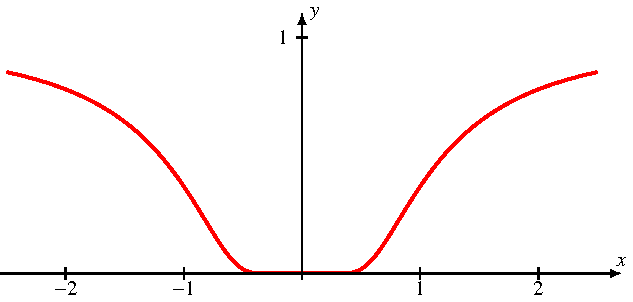
\includegraphics{chapters/080-funktionentheorie/images/nonanalytic.pdf}
\caption{Beispiel einer beliebig oft stetig differenzierbaren Funktion,
deren Ableitungen in $x=0$ alle verschwinden.
Die zugehörige Taylor-Reihe ist die Nullfunktion, sie hat nichts mit der
Funktion zu tun.
\label{buch:funktionentheorie:fig:nonanalytic}}
\end{figure}

\begin{beispiel}
\label{buch:funktionentheorie:beispiel:nichtanalytisch}
Wir betrachten die Funktion
\[
f\colon \mathbb{R}\to\mathbb{R}
:
x \mapsto
\begin{cases}
e^{-1/x^2}&\qquad x\ne 0\\
0&\qquad x=0.
\end{cases}
\]
Der Graph $y=f(x)$ ist in Abbildung~\ref{buch:funktionentheorie:fig:nonanalytic}
dargestellt.

Die ersten zwei Ableitungen der Funktion $f$ sind
\begin{align*}
f'(x) &= \frac{2e^{-1/x^2}}{x^3} = \frac{2}{x^3}\cdot f(x)
\\
f''(x) &= \frac{(4-6x^2) e^{-1/x^2}}{x^6} = \frac{4-6x^2}{x^6}\cdot f(x)
\\
&\dots
\end{align*}
Man kann vermuten, dass alle
Ableitungen Funktionen der Form
\begin{equation}
F(x) = \frac{p(x)}{x^n} \cdot f(x),
\label{buch:funktionentheorie:eqn:nonanalytic:form}
\end{equation}
sind,
wobei $p(x)$ ein Polynom ist.
Leitet man eine solche Funktion nach $x$ ab, erhält man
\begin{align*}
\frac{d}{dx} F(x)
&=
\frac{\frac{d}{dx}(p(x)f(x)) x^n - nx^{n-1}p(x)f(x)}{x^{2n}}
\\
&=
\frac{p'(x)f(x) + p(x)f'(x) - nx^{n-1}p(x)f(x)}{x^{2n}} 
\\
&=
\frac{p'(x) + p(x)(2/x^3) - nx^{n-1}p(x)}{x^{2n}} \cdot f(x)
\\
&=
\frac{x^3p'(x)+2p(x)-nx^{n-1}p(x)}{x^{2n+3}}\cdot f(x).
\end{align*}
Dies ist wieder eine Funktion der
Form~\eqref{buch:funktionentheorie:eqn:nonanalytic:form}.

Der Faktor $f(x)=e^{-1/x^2}$ von $F(x)$ geht für $x\to 0$ exponentiell
schnell gegen $0$, schneller als der Nenner $x^n$ gegen $0$ gehen
kann. 
Der Grenzwert $x\to 0$ einer Funktion der 
Form~\eqref{buch:funktionentheorie:eqn:nonanalytic:form}
ist daher immer
\[
\lim_{x\to 0}  F(x) =0.
\]
Damit ist gezeigt, dass alle Ableitungen $f^{(n)}(0)=0$ sind.
Die Taylorreihe von $f(x)$ ist daher die Nullfunktion.
\end{beispiel}

Die Klasse der Funktionen, die sich durch ihre Taylor-Reihe darstellen
lassen, zeichnet sich also durch besondere Eigenschaften aus, die in
der folgenden Definition zusammengefasst werden.

\index{analytisch in einem Punkt}%
\index{analytisch}%
\begin{definition}
Eine auf einem offenen Intervall $I\subset \mathbb {R}$ definierte Funktion
$f\colon U\to\mathbb{R}$ heisst {\em analytisch im Punkt  $x_0\in I$}, wenn
es eine in einer Umgebung von $x_0$ konvergente Potenzreihe
\[
\sum_{k=0}^\infty a_k(x-x_0)^k = f(x)
\]
gibt.
Sie heisst {\em analytisch}, wenn sie analytisch ist in jedem Punkt von $I$.
\end{definition}

Es ist wohlbekannt aus der elementaren Theorie der Potenzreihen, dass
eine analytische Funktion beliebig oft differenzierbar ist und dass
die Potenzreihe im Punkt $x_0$ die Taylor-Reihe sein muss.
Ausserdem sidn Summen, Differenzen und Produkte von analytischen Funktionen
wieder analytisch.

Für eine komplexe Funktion lässt sich der Begriff der
analytischen Funktion genau gleich definieren.

\begin{definition}
Eine in einer offenen Teilmenge $U\subset \mathbb{C}$ definierte Funktion
$f\colon U\to\mathbb{C}$ heisst {\em analytisch im Punkt $z_0\in U$}, wenn
es eine in einer Umgebung von $z_0$ konvergente Potenzreihe
\[
\sum_{k=0}^\infty a_k(z-z_0)^k = f(z)
\]
gibt.
Sie heisst {\em analytisch}, wenn sie analytisch ist in jedem Punkt von $U$.
\end{definition}

Die Verwendung einer offenen Teilmenge $U\subset\mathbb{C}$ ist wesentlich,
denn die Funktion $f\colon z\mapsto \overline{z}$ kann in jedem Punkt
$x_0\in\mathbb{R}$
der reellen Achse $\mathbb{R}\subset\mathbb{C}$ durch die Potenzreihe 
$f(x) = x_0 + (x-x_0)$ dargestellt werden.
Es gibt aber keine Potenzreihe, die $f(z)$ in einer offenen Teilmenge
von $\mathbb{C}$ gegen $f(z)=\overline{z}$ konvergiert.

%
% Der Konvergenzradius einer Potenzreihe
%
\subsection{Konvergenzradius
\label{buch:funktionentheorie:subsection:konvergenzradius}}
In der Theorie der Potenzreihen, die man in einem grundlegenden
Analysiskurs lernt, wird auch genauer untersucht, wie gross
eine Umgebung des Punktes $z_0$ ist, in der die Potenzreihe
im Punkt $z_0$ einer analytischen Funktion konvergiert.

\begin{satz}
\label{buch:funktionentheorie:satz:konvergenzradius}
Die Potenzreihe
\[
f(z) = \sum_{k=0}^\infty a_0(z-z_0)^k
\]
ist konvergent auf einem Kreis mit Radius $\varrho$ und
\[
\frac{1}{\varrho}
=
\limsup_{n\to\infty} \sqrt[k]{|a_k|}.
\]
Falls $a_k\ne 0$ für alle $k$ und der folgende Grenzwert existiert,
dann gilt auch
\[
\varrho = \lim_{n\to\infty} \biggl| \frac{a_n}{a_{n+1}}\biggr|.
\]
\end{satz}

\begin{definition}
\label{buch:funktionentheorie:definition:konvergenzradius}
\index{Konvergenzradius}%
Der in Satz~\ref{buch:funktionentheorie:satz:konvergenzradius}
Radius $\varrho$ des Konvergenzkreises heisst {\em Konvergenzradius}.
\end{definition}

Man kann auch zeigen, dass der Konvergenzkreis immer so gross ist,
dass auf seinem Rand ein Wert $z$ liegt, für den die Potenzreihe nicht
konvergiert.


%
% cauchy.tex
%
% (c) 2021 Prof Dr Andreas Müller, OST Ostschweizer Fachhochschule
%
\section{Cauchy-Integral
\label{buch:funktionentheorie:section:cauchy}}
\rhead{Cauchy-Integral}
In Abschnitt~\ref{buch:funktionentheorie:section:holomorph} hat sich
bereits gezeigt, dass komplexe Differenzierbarkeit einer komplexen
Funktion weit mehr Einschränkungen auferlegt als reelle Differenzierbarkeit.
Sowohl der Real- wie auch der Imaginärteil müssenharmonische Funktionen
sein.
In diesem Abschnitt wird die Cauchy-In\-te\-gral\-formel etabliert, die 
sogar zeigt, dass eine komplex differenzierbare Funktion bereits durch 
die Werte auf dem Rand eines einfach zusammenhängenden Gebietes
gegeben ist, beliebig oft differenzierbar ist und ausserdem immer
analytisch ist.

%
% Wegintegrale und die Cauchy-Formel
%
\subsection{Wegintegrale\label{subsection:wegintegrale}}
Das Finden einer Stammfunktion, die Integration, ist die Grundtechnik,
\index{Stammfunktion}%
mit der man den Übergang von lokaler Information in Form von Ableitungen,
zu globaler Information über reelle Funktionen vollzieht.
Sie liefert aus der Steigung zwischen zwei Punkten $x_0$ und $x$ den
Funktionswert mittels
\[
f(x)=f(x_0)+\int_{x_0}^xf'(\xi)\,d\xi.
\]
Bei einer reellen Funktion gibt es nur eine Richtung, entlang der man
integrieren könnte.

Auch in der komplexen Ebene erwarten wir eine Formel
\[
f(z) = f(z_0) + \int_{z_0}^z f'(\zeta)\,d\zeta.
\]
In der komplexen Ebene gibt es aber beliebig viele Wege, mit denen die
Punkte $z_0$ und $z$ verbunden werden können.
Der Wert von $f(z)$ muss also durch Integration entlang eines speziell
gewählten Weges $\gamma$
\[
f(z) = f(z_0) + \int_{\gamma} f'(\zeta)\,d\zeta
\]
bestimmt werden.
Es muss also zunächst geklärt werden, wie ein solches Wegintegral
überhaupt zu verstehen und zu berechnen ist.
Dann gilt es zu untersuchen, inwieweit diese Konstruktion unabhängig
von der Wahl des Weges ist.
Für komplex differenzierbare Funktionen wird sich eine sehr erfolgreiche
Theorie ergeben.

%
% Wegintegrale
%
\subsubsection{Definition des Wegintegrals}
Ein Weg in der komplexen Ebene ist eine Abbildung
\index{Abbildung}%
\[
\gamma\colon [a,b]\to\mathbb C: t\mapsto \gamma(t).
\]
Wir verlangen für unsere Zwecke zusätzlich, dass $\gamma$ differenzierbar
ist.
Dann können wir für jede beliebige Funktion das Wegintegral definieren.

\begin{definition}
Sei $\gamma\colon[a,b]\to\mathbb C$ ein Weg in $\mathbb C$ und $f(z)$
eine stetige komplexe Funktion, dann heisst
\[
\int_{\gamma} f(z)\,dz = \int_a^bf(\gamma(t)) \gamma'(t)\,dt
\]
das {\em Wegintegral} von $f(z)$ entlang der Kurve $\gamma$.
\index{Wegintegral}
\end{definition}

\begin{beispiel}
Man berechne das Wegintegral der Funktion $f(z)=z^n$ entlang des
Weges
$\gamma(t)=1+t+it^2$
für $t\in[0,1]$.

Die Definition besagt
\begin{align*}
\int_\gamma f(z)\,dz
&=
\int_0^1 f(\gamma(t))\gamma'(t)\,dt
=
\int_0^1 \gamma(t)^n \gamma'(t)\,dt
=
\int_0^1 \frac{d}{dt}\frac{\gamma(t)^{n+1}}{n+1}\,dt
\\
&=
\biggl[\frac{\gamma(t)^{n+1}}{n+1}\biggr]_0^1
=
\frac{(2+i)^{n+1}}{n+1}-\frac{1^{n+1}}{n+1}
=
\frac{(2+i)^{n+1}-1}{n+1}.
\end{align*}
Man stellt in diesem Beispiel auch fest, dass das Integral offenbar
unabhängig ist von der Wahl des Weges, es kommt einzig auf die
beiden Endpunkte an:
\[
\int_\gamma z^n \,dz = \frac1{n+1}\bigl(\gamma(1)^{n+1}-\gamma(0)^{n+1}\bigr).
\]
\end{beispiel}

\begin{beispiel}
Wir berechnen als Beispiel das Wegintegral der Funktion $f(z)=1/z$ entlang
eines Halbkreises von $1$ zu $-1$.
Es gibt zwei verschiedene solche Halbkreise:
\begin{equation*}
\begin{aligned}
\gamma_+(t)&=e^{it},&t&\in[0,\pi]
\\
\gamma_-(t)&=e^{-it},&t&\in[0,\pi]
\end{aligned}
\end{equation*}
Wir finden für die Wegintegrale
\begin{align*}
\int_{\gamma_+}\frac1z\,dz
&=
\int_0^\pi \frac1{e^{it}}ie^{it}\,dt=i\int_0^\pi\,dt=i\pi,
\\
\int_{\gamma_-}\frac1z\,dz
&=
-\int_0^\pi \frac1{e^{-it}}ie^{-it}\,dt=-i\int_0^\pi\,dt=-i\pi.
\end{align*}
Das Wegintegral zwischen $1$ und $-1$ hängt also mindestens für diese
spezielle Funktion $f(z)=1/z$ von der Wahl des Weges ab.
\end{beispiel}

Wie Wahl der Parametrisierung der Kurve hat keinen Einfluss auf den
Wert des Wegintegrals.

\begin{satz}
Seien $\gamma_1(t), t\in[a,b],$ und $\gamma_2(s),s\in[c,d]$
verschiedene Parametrisierungen
\index{Parametrisierung}%
der gleichen Kurve, es gebe also eine Funktion $t(s)$ derart, dass
$\gamma_1(t(s))=\gamma_2(s)$.
Dann ist
\[
\int_{\gamma_1}f(z)\,dz
=
\int_{\gamma_2}f(z)\,dz.
\]
\end{satz}

\begin{proof}[Beweis]
Wir verwenden die Definition des Wegintegrals
\begin{align*}
\int_{\gamma_1} f(z)\,dz
&=
\int_a^b f(\gamma_1(t))\,\gamma_1'(t)\,dt
=
\int_c^d f(\gamma_1(t(s))\,\underbrace{\gamma_1'(t(s)) t'(s)}_{\displaystyle
=\frac{d}{ds}\gamma_1(t(s))}\,ds
\\
&=
\int_c^d f(\gamma_2(s)\,\gamma_2'(s)\,ds
=
\int_{\gamma_2}f(z)\,dz.
\end{align*}
Beim zweiten Gleichheitszeichen haben wir die Formel für die
Variablentransformation $t=t(s)$ in einem Integral verwendet.
\index{Variablentransformation}%
\end{proof}

Wir erwarten, dass das Wegintegral ähnlich wie das Integral reeller
Funktionen eine Art ``Umkehroperation'' zur Ableitung ist.
Wir untersuchen daher den Fall, dass $f(z)$ eine komplexe Stammfunktion $F(z)$
hat, also $f(z)=F'(z)$.
Wir berechnen das Wegintegral entlang des Weges $\gamma$:
\begin{align*}
\int_{\gamma}f(z)\,dz
&=
\int_a^bf(\gamma(t))\,\gamma'(t)\,dt
=
\int_a^bF'(\gamma(t))\,\gamma'(t)\,dt
=
\int_a^b\frac{d}{dt}F(\gamma(t))\,dt
=
F(\gamma(a))-F(\gamma(b))
\end{align*}
Dies ist genau die Formel, die man als den Hauptsatz der Infinitesimalrechnung
kennt.
Trotzdem ist die Situation hier etwas anders.
In der reellen Infinitesimalrechnung war die Existenz einer Stammfunktion
durch das Integral gesichert, man konnte mit
\[
F(x)=\int_a^xf(\xi)\,d\xi
\]
immer eine Stammfunktion angeben.
Im komplexen Fall können wir natürlich auch versuchen, eine Stammfunktion
mit Hilfe von
\[
F(z)=\int_{\gamma_z} f(\zeta)\,d\zeta
\]
zu definieren.
Dabei muss allerdings $\gamma_z$ ein Weg sein, der im Punkt $z$ endet,
und wir wissen noch nicht einmal, ob die Wahl des Weges eine Rolle
spielt.
Bevor wir also sicher sein können, dass eine Stammfunktion existiert,
müssen wir zeigen, dass das Wegintegral einer komplex differenzierbaren
Funktion zwischen zwei Punkten nicht von der Wahl des Weges abhängt,
der die beiden Punkte verbindet.
Dazu ist notwendig, geschlossene Wege genauer zu betrachten.

%
% Wegintegrale führen auf analytische Funktionen
%
\subsubsection{Wegintegrale führen auf analytische Funktionen}
\begin{figure}
\centering
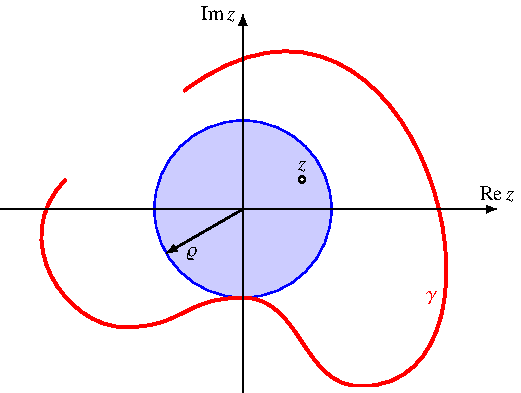
\includegraphics{chapters/080-funktionentheorie/images/integralanalytisch.pdf}
\caption{Pfad und Konvergenzradius für den Nachweis, dass Wegintegrale
auf analytische Funktionen führen (Satz~\ref{komplex:integralanalytisch}).
\label{komplex:integralanalytischpfad}}
\end{figure}
Mit Wegintegralen kann man aus stetigen Funktionen neue Funktionen
konstruieren.
Die folgende Konstruktion liefert überraschenderweise immer
analytische Funktionen.
\begin{satz}
\label{komplex:integralanalytisch}
Sei $\gamma\colon [a,b]\to\mathbb C$ ein Weg in $\mathbb C$, der nicht
durch den Nullpunkt verläuft, und $g$ eine stetige Funktion
auf $\gamma([a,b])$ (Abbildung~\ref{komplex:integralanalytischpfad}).
Dann ist die Funktion
\[
f(z) = \frac1{2\pi i}\int_\gamma \frac{g(x)}{x-z}\,dx
\]
in einer Umgebung des Nullpunktes analytisch:
\[
f(z) = \sum_{k=0}^\infty c_k z^k,\qquad
\text{mit\quad}
c_k=\frac1{2\pi i}\int_\gamma \frac{g(x)}{x^{k+1}}\,dx.
\]
Der Konvergenzradius $\varrho$ dieser Reihe ist der minimale Abstand der
Kurve $\gamma$ vom Nullpunkt.
\end{satz}

\begin{proof}[Beweis]
Zunächst schreiben wir
\begin{equation}
\frac{1}{x-z}
=
\frac1x\cdot \frac{1}{1-\displaystyle\frac{z}{x}}
=
\frac1x\cdot \sum_{k=0}^\infty \biggl(\frac{z}{x}\biggr)^k
=
\sum_{k=0}^\infty \frac{z^k}{x^{k+1}}.
\label{komplex:georeihe}
\end{equation}
Damit können wir jetzt die Funktion $f(z)$ berechnen:
\begin{align*}
f(z)
&=
\frac1{2\pi i} \int_{\gamma} \frac{g(x)}{x-z}\,dx
=
\frac1{2\pi i} \int_{\gamma} \sum_{k=0}^\infty \frac{z^k}{x^{k+1}}g(x)\,dx
=
\sum_{k=0}^\infty
\underbrace{\biggl(\frac1{2\pi i} \int_{\gamma} \frac{g(x)}{x^{k+1}}\,dx\biggr)}_{\displaystyle =c_k}
z^k
=
\sum_{k=0}^\infty c_kz^k.
\end{align*}
Wir müssen uns noch die Konvergenz dieser Reihen überlegen.
Wenn $z<\varrho$ ist, dann ist
\[
\biggl|\frac{z}{x}\biggr| 
=
\frac{|z|}{|x|}
<1,
\]
so dass die geometrische Reihe \eqref{komplex:georeihe} konvergent ist,
daraus lesen wir ab, dass der Konvergenzradius mindestens $\varrho$
ist.
Grösser kann er allerdings auch nicht sein, da für $|z|\ge \varrho$
das Integral nicht mehr definiert sein muss.
Nimmt man nämlich einen Punkt von $g([a,b])$ für $z$ wird der Integrand
unendlich gross.
\end{proof}

Der Satz~\ref{komplex:integralanalytisch} ist nur für Potenzreihen
im Punkt $0$ formuliert, was im Wesentlichen durch die
Umformung~\eqref{komplex:georeihe} bedingt war.
Man kann dies aber auch als Potenzreihe
\[
\frac1{x-z}
=
\frac1{x-z_0-(z-z_0)}
=
\frac1{x-z_0}\cdot\frac1{1-\displaystyle\frac{z-z_0}{x-z_0}}
=
\frac1{x-z_0}\sum_{k=0}^\infty\biggl(\frac{z-z_0}{x-z_0}\biggr)^k
=
\sum_{k=0}^\infty\frac1{(x-z_0)^{k+1}}(z-z_0)^k
\]
im Punkt $z_0$ ausdrücken.
Man bekommt dann die Potenzreihe
\[
f(z) = \sum_{k=1}^\infty c_k(z-z_0)^k,\qquad
\text{mit}\quad
c_k=\frac1{2\pi i}\oint_\gamma\frac{g(x)}{(x-z_0)^{k+1}}\,dx
\]
für das Wegintegral.

\subsubsection{Laurent-Reihen}
\label{sssec:LaurentReihen}
\begin{figure}
\centering
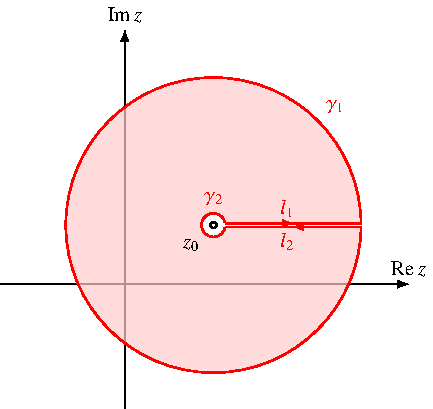
\includegraphics{chapters/080-funktionentheorie/images/laurent.pdf}
\caption{Pfad zur Herleitung der Laurent-Reihe einer Funktion $f(z)$
mit einer Singularität $z_0$.
\label{komplex:laurentpfad}}
\end{figure}%
\index{Laurent-Reihe}%
In Satz~\ref{komplex:integralanalytisch} konnten wir eine Potenzreihe für
solche $z$ konstruieren, deren Betrag kleiner ist als der kleinste Abstand
der Kurve $\gamma$ vom Ursprung.
Dies war notwendig, weil in~\eqref{komplex:georeihe} die geometrische Reihe
nur konvergiert, wenn der Quotient $<1$ ist.
Wenn die Funktion $f(z)$ jedoch eine Singularität im Punkt $z_0$ hat, dann
kann es nicht möglich sein, die Funktion mit einer Potenzreihe zu
beschreiben.

Wir verwenden daher den speziellen Pfad in Abbildung~\ref{komplex:laurentpfad}.
Er führt in einem grossen Kreis $\gamma_1$ um den Punkt $z_0$ herum,
dann folgt ein zur $x$-Achse paralleler Abschnitt, der bis zum kleinen
Kreis $\gamma_2$ führt.
Nach Durchlaufen des kleinen Kreises $\gamma_2$ im Uhrzeigersinn folgt wieder
ein zur $x$-Achse paralleles Stück zurück zum grossen Kreis.
Da die geraden Stücke zweimal in entgegegengesetzer Richtung durchlaufen
werden, heben sie sich weg.
Ein Wegintegral entlang $\gamma$ zerfällt daher in eine Differenz
\[
\oint_\gamma\dots\,dz
=
\oint_{\gamma_1}\dots\,dz
-
\oint_{\gamma_2}\dots\,dz
\]
von Wegintegralen entlang $\gamma_1$ und $\gamma_2$.

Der äussere Pfad $\gamma_1$ gibt wie in Satz~\ref{komplex:integralanalytisch}
Anlass zu einer Potenzreihe in $(z-z_0)$.
Der innere Pfad $\gamma_2$ kann aber nicht so behandelt werden, da $z$ immer
weiter von $z_0$ entfernt als die Punkte auf $\gamma_2$.
Allerdings ist $|x/z| < 1$ für Punkte auf $\gamma_2$, wir müssen daher
die geometrische Reihe auf $x/z$ anwenden:
\begin{align*}
\frac{1}{x-z}
&=
\frac{1}{x-z_0-(z-z_0)}
=
\frac{1}{z-z_0}
\cdot
\frac{1}{\displaystyle\frac{x-z_0}{z-z_0}-1}
=
-\sum_{k=0}^\infty \frac{(x-z_0)^k}{(z-z_0)^{k+1}}.
\end{align*}
Das Integral entlang der Kurve $\gamma_2$ kann also als Reihe in $1/(z-z_0)$
entwickelt werden:
\begin{align*}
f_2(z)
&=
\frac{1}{2\pi i}\int_{\gamma_2} \frac{g(x)}{x-z}\,dx
=
\frac{1}{2\pi i}\int_{\gamma_2}\sum_{k=0}^\infty
\frac{(x-z_0)^k}{(z-z_0)^{k+1}}\,dx
\\
&=
\sum_{k=0}^\infty
\biggl(
\underbrace{\frac1{2\pi i}\int_{\gamma_2} (x-z_0)^kg(x)\,dx
}_{\displaystyle =d_{k+1}}
\biggr)
\frac1{(z-z_0)^{k+1}}
=\sum_{k=1}^\infty \frac{d_k}{(z-z_0)^k}.
\end{align*}
Zusammen mit der vom Integral entlang $\gamma_1$ herrührenden Reihe finden
wir den Satz
\begin{satz}
\label{komplex:laurentreihe}
Ist $g(z)$ eine entlang der Kurve $\gamma$ wie in
Abbildung~\ref{komplex:laurentpfad} definierte stetige Funktion, dann gilt
\[
f(z)=\frac1{2\pi i}\oint_{\gamma} \frac{f(x)}{x-z}\,dx
=
\sum_{k=0}^{\infty} c_k(z-z_0)^k-\sum_{k=1}^\infty \frac{d_k}{(z-z_0)^k},
\]
wobei die Koeffizienten $c_k$ und $d_k$ gegeben sind durch
\[
\begin{aligned}
c_k&=\frac1{2\pi i}\oint_{\gamma_1} \frac{g(x)}{x-z_0}\,dx
&&
\text{und}
&
d_k&=\frac1{2\pi i}\oint_{\gamma_2} g(x)x^{k-1}\,dx.
\end{aligned}
\]
\end{satz}

\begin{definition}
Eine Reihe der Form
\[
\sum_{k=-\infty}^\infty a_k(z-z_0)^k
\]
heisst {\em Laurent-Reihe }
im Punkt $z_0$.
\end{definition}


%
% Geschlossene Wege
%
\subsubsection{Geschlossene Wege}
\begin{definition}
Ein Weg $\gamma\colon[a,b]\to\mathbb C$ heisst {\em geschlossen}, wenn
$\gamma(a)=\gamma(b)$.
\index{geschlossener Weg}
Das Integral entlang eines geschlossenen Weges hängt nicht von der
Parametrisierung ab und wird zur Verdeutlichung mit
\[
\int_{\gamma}f(z)\,dz
=
\oint_{\gamma}f(z)\,dz
\]
bezeichnet.
\end{definition}

\begin{beispiel}
Wir berechnen das Integral von $f(z)=z^n$ entlang des Einheitskreises,
den wir mit $\gamma(t)=e^{it},t\in[0,2\pi]$ parametrisieren.
Die Definition liefert:
\begin{align*}
\oint_{\gamma}f(z)\,dz
&=
\int_0^{2\pi}e^{int}ie^{it}\,dt
=
i\int_0^{2\pi}e^{i(n+1)t}\,dt
\end{align*}
Für $n=-1$ ist dies das Integral einer konstanten Funktion, also
\[
\oint_{\gamma}\frac1z\,dz=2\pi i.
\]
Für $n\ne -1$ kann man eine Stammfunktion von $e^{i(n+1)t}$
verwenden:
\[
\oint_{\gamma}f(z)\,dz
=
i\left[\frac1{i(n+1)}e^{i(n+1)t}\right]_0^{2\pi}
=0,
\]
weil $e^{i(n+1)t}$ periodisch ist mit Periode $2\pi$.
\end{beispiel}
Das Beispiel zeigt, dass ein Wegintegral der Potenzfunktionen,
aller Polynome und schliesslich aller konvergenten Potenzreihen
über einen geschlossenen Weg verschwinden.
Es zeigt aber auch, dass das Wegintegral über einen geschlossenen
Weg nicht zu verschwinden braucht, wie das Beispiel $f(z)=1/z$
zeigt.
Letztere Funktion unterscheidet sich von den Potenzfunktionen allerdings
dadurch, dass sie im Nullpunkt nicht definiert ist.

\begin{satz}
Sei $f(z)$ eine in einem zusammenhängenden Gebiet $\Omega\subset\mathbb C$
definierte komplexe Funktion, für die das Wegintegral über jeden
geschlossenen Weg verschwindet.
Dann hat $f(z)$ eine komplexe Stammfunktion $F(z)$.
\end{satz}

\begin{proof}[Beweis]
Wir wählen einen beliebigen Punkt $z_0\in\Omega$ definieren die
komplexe Stammfunktion mit Hilfe des Wegintegrals
\[
F(z)=\int_{\gamma_z} f(\zeta)\,d\zeta,
\]
wobei $\gamma_z$ ein beliebiger Weg ist, der $z_0$ mit $z$ verbindet.

Wir müssen uns davon überzeugen, dass die Wahl des Weges keinen Einfluss
auf $F(z)$ hat.
Dazu seien $\gamma_1$ und $\gamma_2$ zwei verschiedene Wege, die
$z_0$ mit $z$ verbinden.
Da die Parametrisierung der Wege keinen Einfluss auf das Wegintegral haben,
nehmen wir an, dass beide Wege auf dem Intervall $[0,1]$ definiert sind.

Jetzt konstruieren wir einen geschlossene Weg $\gamma$ durch die
Definition:
\[
\gamma\colon[0,2]\to\mathbb C:t\mapsto
\begin{cases}
\gamma_1(t)&\qquad 0\le t\le 1\\
\gamma_2(2-t)&\qquad 1\le t\le 2
\end{cases}
\]
Der Weg $\gamma$ besteht aus $\gamma_1$ und dem in umgekehrter Richtung
durchlaufenen Weg $\gamma_2$, denn an der Stelle $t=1$ passen die
beiden Teilwege nahtlos zusammen: $\gamma_1(1)=\gamma_2(1)=\gamma_2(2-1)$.
Wegen $\gamma(2)=\gamma_2(2-2)=\gamma_2(0)=\gamma_1(0)$ ist der
Weg geschlossen.
Nach Voraussetzung ist verschwindet das Wegintegral über $\gamma$.
Es folgt
\begin{align*}
0
&=
\int_{\gamma}f(z)\,dz
\\
&=
\int_0^1 f(\gamma_1(t))\gamma_1'(t)\,dt
+ \int_1^2f(\gamma_2(2-t))\frac{d}{dt}\gamma_2(2-t)\,dt
\\
&=
\int_0^1 f(\gamma_1(t))\gamma_1'(t)\,dt
- \int_1^2f(\gamma_2(2-t))\gamma_2'(2-t)\,dt
\\
&=
\int_0^1 f(\gamma_1(t))\gamma_1'(t)\,dt
- \int_0^1f(\gamma_2(s))\gamma_2'(s)\,ds
\\
&=
\int_{\gamma_1}f(z)\,dz - \int_{\gamma_2}f(z)\,dz
\\
\Rightarrow\qquad
\int_{\gamma_2}f(z)\,dz&=\int_{\gamma_1}f(z)\,dz.
\end{align*}
Da die Wahl des Weges keine Rolle spielt, ist $F(z)$ wohldefiniert.
\end{proof}

Die Bedingung des eben bewiesenen Satzes ist nicht wirklich nützlich,
sie ist kaum nachprüfbar.
Es braucht also zusätzliche Anstrengungen um genügend viele
Funktionen zu finden, welche die Eigenschaft haben, dass Wegintegrale
über geschlossene Wege verschwinden.
Wir zielen dabei auf den folgenden Satz hin:
\begin{satz}[Cauchy]
Ist $f(z)$ eine in einem Gebiet $\Omega\subset\mathbb C$ definierte
komplex differenzierbare Funktion, und ist $\gamma$ ein im Gebiet
$\Omega$ auf einen Punkt zusammenziehbarer geschlossener Weg, dann gilt
\[
\oint_{\gamma}f(z)\,dz=0.
\]
Ist insbesondere $\Omega$ {\em einfach zusammenhängend}
\index{einfach zusammenhangend@einfach zusammenhängend}%
\index{zusammenziehbar}%
(d.~h.~jeder geschlossene Weg lässt sich in einen Punkt zusammenziehen),
dann verschwindet das Wegintegral von $f(z)$ über jeden geschlossenen
Weg in $\Omega$.
\index{einfach zusammenhangend@einfach zusammenhängend}
\end{satz}


\begin{proof}[Beweis]
Wir verwenden für den folgenden Beweis den Satz von Green über
\index{Green, Satz von}%
Wegintegrale in der Ebene.
Er besagt, dass für einen geschlossenen Weg $\gamma$ der in der Ebene
das Gebiet $D$ berandet, und zwei Funktionen $L(x,y)$ und $M(x,y)$, gilt
\[
\oint_\gamma(L\,dx + M\,dy)
=
\int_D \biggl(\frac{\partial M}{\partial x}
-\frac{\partial L}{\partial y}\biggr)\,dx\,dy.
\]
Wir berechnen jetzt das Integral einer komplex differenzierbaren Funktion
$f(z)$
\begin{align*}
\oint_\gamma f(z)\,dz
&=
\int (u(x,y)+iv(x,y))(\dot x(t)+i\dot y(t))\,dt
\\
&=
\int u(x,y)\dot x(t) -v(x,y)\dot y(t)\,dt
+
i \int u(x,y)\dot y(t)+v(x,y)\dot x(t)\,dt
\\
&=\oint_\gamma(u\,dx - v\,dy) + i\oint_\gamma(v\,dx + u\,dy)
\\
&=
\int_D
\underbrace{-\frac{\partial v}{\partial x}}_{\displaystyle=\frac{\partial u}{\partial y}}
-\frac{\partial u}{\partial y}
\,dx\,dy
+i
\int_D
\underbrace{\frac{\partial u}{\partial x}}_{\displaystyle=\frac{\partial v}{\partial y}}
-\frac{\partial v}{\partial y}\,dx\,dy
=0.
\end{align*}
Dabei haben wir auf der dritten Zeile den Satz von Green angewendet,
und auf der letzten Zeile die Cauchy-Riemann-Differentialgleichungen.
\end{proof}

\subsection{Die Cauchy-Integralformel}
\index{Cauchy-Integralformel}%
Sei jetzt $f(z)$ eine komplex differenzierbare Funktion.
Dann ist auch die Funktion
\[
g(z)=\frac{f(z)}{z-a}
\]
komplex differenzierbar für $z\ne a$.
Insbesondere ist der Wert des Wegintegrals von $g(z)$ entlang
eines geschlossenen Pfades um den Punkt $a$ unabhängig von der Wahl
des Weges.
Zum Beispiel könnten wir das Wegintegral mit Hilfe eines kleinen Kreises
um $a$ mit Radius $r$ mit der Parametrisierung
\[
t\mapsto \gamma(t)=a+re^{it},\quad t\in[0,2\pi]
\]
berechnen.
Die Rechnung ergibt
\begin{align*}
\oint_\gamma \frac{f(z)}{z-a}\,dz
&=
\int_0^{2\pi} \frac{f(a+re^{it})}{re^{it}}ire^{it}\,dt
=
i\int_0^{2\pi} f(a+re^{it})\,dt
\end{align*}
Da $f(z)$ komplex differenzierbar ist, können wir $f(z)$ approximieren
durch $f(z)=f(a)+f'(a)(z-a)+o(z-a)$, also
\begin{align*}
\oint_{\gamma} \frac{f(z)}{z-a}\,dz
&=
i\int_0^{2\pi}f(a) + f'(a)re^{it}+o(r)\,dt
\\
&=
f(a)i\int_0^{2\pi}\,dt
+ irf'(a)\int_0^{2\pi} e^{it}\,dt + i\int_0^{2\pi}o(r)\,dt
\\
&=
2\pi i f(a) + irf'(a)\underbrace{\left[\frac1{i}e^{it}\right]_0^{2\pi}}_{\displaystyle=0}+o(r)
\\
&=2\pi i f(a)+o(r).
\end{align*}
Da das Wegintegral einer komplex differenzierbaren Funktion aber unabhängig
vom Weg und damit vom Radius $r$ sein muss, folgt
\[
\oint_\gamma \frac{f(z)}{z-a}\,dz=2\pi i f(a).
\]
Wir haben damit den folgenden Satz bewiesen:

\begin{satz}[Cauchy]
Ist $\gamma$ ein geschlossener Weg in der komplexen Ebene, die ein
Gebiet umrandet, in dem die komplexe Funktion $f(z)$ komplex
differenzierbar ist, dann gilt
\[
f(a)=\frac{1}{2\pi i}\oint_{\gamma}\frac{f(z)}{z-a}\,dz.
\]
Insbesondere sind die Werte einer komplex differenzierbaren Funktion
im Inneren eines Gebietes durch die Werte auf dem Rand bereits vollständig
bestimmt.
\end{satz}

\subsubsection{Ableitungen und Cauchy-Formel}
Sei $f(z)$ eine komplex differenzierbare Funktion, als Definitionsgebiet
nehmen wir der Einfachheit halber einen Kreis vom Radius $r$ um den Nullpunkt,
sein Rand ist die Kurve $\gamma$.
Durch Ableiten der Cachyschen Integralformel finden wir
\begin{align*}
f(z)
&=
\frac1{2\pi i}\oint_{\gamma}\frac{f(\zeta)}{\zeta-z}\,d\zeta
\\
f'(z)
&=
\frac1{2\pi i}\oint_{\gamma}\frac{f(\zeta)}{(\zeta-z)^2}\,d\zeta
\\
f'' (z)
&=
\frac1{2\pi i}\oint_{\gamma}2\frac{f(\zeta)}{(\zeta-z)^3}\,d\zeta
\\
f'''(z)
&=
\frac1{2\pi i}\oint_{\gamma}2\cdot 3\frac{f(\zeta)}{(\zeta-z)^4}\,d\zeta
\\
&\vdots
\\
f^{(k)}(z)
&=
\frac{k!}{2\pi i}\oint_{\gamma}\frac{f(\zeta)}{(\zeta-z)^{k+1}}\,d\zeta.
\end{align*}
Es folgt

\begin{satz}
Eine komplex differenzierbare Funktion ist beliebig oft differenzierbar.
\end{satz}

\subsubsection{Komplex differenzierbare Funktionen sind analytisch}
Wir haben früher gesehen, dass Wegintegrale auf analytische Funktionen
führen.
Andererseits zeigt das Cauchy-Integral, dass komplex differenzierbare
Funktionen durch genau die Integrale bestimmt sind, die in den
Reihenentwicklungen in Satz~\ref{komplex:integralanalytisch} auftraten.
Diese Resultate können wir im folgenden Satz zusammenfassen.

\begin{satz}
Eine komplex differenzierbare Funktion $f(z)$, die in einer Kreisscheibe
vom Radius $r$ um den Punkt $z_0$ definiert ist, ist analytisch.
Ihre Potenzreihenentwicklung
\[
f(z)=\sum_{k=0}^na_k(z-z_0)^k
\]
hat die Koeffizienten
\[
a_k=\frac1{2\pi i}\int_{\gamma}\frac{f(z)}{(z-z_0)^{k+1}}\,dz,\quad
k\ge 0.
\]
\end{satz}

\begin{proof}[Beweis]
Da $f$ komplex differenzierbar ist, gilt
\[
f(z)=\frac1{2\pi i}\oint_\gamma \frac{f(\zeta)}{\zeta-z}\,d\zeta.
\]
In Satz~\ref{komplex:integralanalytisch} wurde gezeigt, dass $f(z)$
analytisch ist, und dass die Koeffizienten der Potenzreihe von
der verlangten Form sind.
\end{proof}

Für eine komplexe Funktion, die im Punkt $z_0$ eine Singularität hat,
also in einer Umgebung von $z_0$ ohne den Punkt $z_0$ definiert ist,
können wir das Resultat aus Satz~\ref{komplex:laurentreihe} verwenden,
und zum folgenden analogen Resultat gelangen:

\begin{satz}
Eine komplex differenzierbare Funktion $f(z)$, die in einer Kreisscheibe
vom Radius $r$ um den Punkt $z_0$ mit Ausnahme des Punktes $z_0$
definiert ist, kann in eine konvergente Laurent-Reihe
\[
f(z)=\sum_{k=-\infty}^{\infty} c_k(z-z_0)^k
\]
entwickelt werden, deren Koeffizienten durch
\[
c_k = \frac1{2\pi i}\oint_\gamma \frac{f(\zeta)}{(z-z_0)^{k+1}}\,d\zeta,\qquad k\in\mathbb Z
\]
gegeben sind.
\end{satz}


%
% fortsetzung.tex
%
% (c) 2021 Prof Dr Andreas Müller, OST Ostschweizer Fachhochschule
%
\section{Analytische Fortsetzung
\label{buch:funktionentheorie:section:fortsetzung}}
\rhead{Analytische Fortsetzung}

Wir haben schon gesehen, dass eine reelle Funktion, die in einem
Punkte eine konvergente
Potenzreihe besitzt, auf natürliche Weise auch als komplexe Funktion
betrachtet werden kann, indem man komplexe Argumente in der Potenzreihe
zulässt.
Die neue komplexe Funktion ist ein einem Kreis um den Punkt
konvergent.
Mit Hilfe der Potenzreihe kann man also immer eine Funktion auf ein
Kreisgebiet ausdehen.
Dieser Abschnitt untersucht die Frage, ob man diese Idee auch auf
noch grössere Gebiete ausdehnen kann.
\subsection{Analytische Fortsetzung mit Potenzreihen}
\begin{figure}
\centering
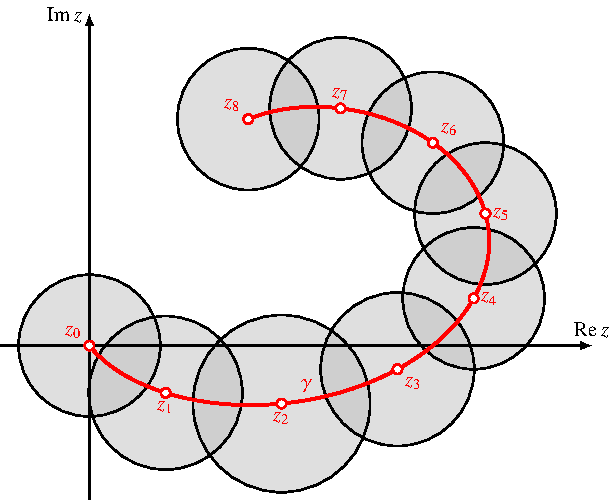
\includegraphics{chapters/080-funktionentheorie/images/forts.pdf}
\caption{Analytische Fortsetzung einer komplexen Funktion entlang einer
Kurve $\gamma$.
\label{komplex:fortsetzung}}
\end{figure}
Eine komplex differenzierbare Funktion $f(z)$ ist immer darstellbar als
Potenzreihe, und ist daher analytisch.
So kann zum Beispiel die Funktion $1/z$ als Potenzreihe um jeden
beliebigen Punkt $z_0$ entwickelt werden:
\begin{align}
f(z)
&=
\frac1z
=
\frac1{z_0-(z_0-z)}
=
\frac1{z_0}\cdot
\frac1{1-\displaystyle\frac{z_0-z\mathstrut}{z_0\mathstrut}}
=
\frac1{z_0}\sum_{k=0}^{\infty} \biggl(\frac{z_0-z\mathstrut}{z_0\mathstrut}\biggr)^k
=
\sum_{k=0}^{\infty} \frac{(-1)^k}{z_0^{k+1}} (z-z_0)^k,
\label{komplex:1durchreihe}
\end{align}
Die Koeffizienten dieser Potenzreihe sind
\[
a_k=\frac{(-1)^k}{z_0^{k+1}},
\]
und man kann den Konvergenzradius ausrechnen:
\[
\frac1{\varrho}
=
\limsup_{k\to\infty} \root{k}\of{|a_k|} = \lim_{k\to\infty}\frac1{|z_0|^{\frac{k+1}{k}}}
=
\frac1{|z_0|}.
\]
Der Konvergenzradius ist limitiert durch die Singularität bei an der Stelle
$z=0$.

Es gibt also keine einzelne Potenzreihe, die die Funktion $f(z)=\frac1z$ in der
ganzen komplexen Ebene darstellen kann.
Wählt man aber einzelne Punkte $z_0$ und $z_1$ derart, dass der Kreis
um $z_0$ mit Radius $|z_0|$ und der Kreis um $z_1$ mit Radius $|z_1|$
überlappen, dann werden die beiden Potenzreihen im Überlappungsgebiet
die gleichen Werte annehmen.

Man könnte allso eine Kurve $\gamma$ in der komplexen Ebene wählen,
entlang der man in jedem Punkt die Funktion $f(z)$ in eine Potenzreihe
entwickelt.
Liegen zwei Punkte nahe genug auf der Kurve $\gamma$, werden die
Konvergenzkreise der Potenzreihen überlappen, und die Potenzreihen
werden im Überlappungsgebiet die gleichen Werte liefern.

Selbst wenn man eine Funktion $f(z)$ nur in einem Kreis um den Punkt $z_0$
kennt, zum Beispiel durch eine Potenzreihe im Punkt $z_0$, kann man entlang
einer Kurve, die $z_0$ mit $z_1$ verbindet, in jedem Punkt eine Potenzreihe
finden, die mit der Potenzreihe in den Nachbarpunkten übereinstimmt, und
so die Definition der Funktion entlang dieser Kurve auf ein grösseres
Gebiet ausweiten, wie in Abbildung~\ref{komplex:fortsetzung} dargestellt.
Man nennt dies die {\em analytische Fortsetzung} der Funktion $f(z)$
entlange der Kurve $\gamma$.
\index{analytische Fortsetzung}
\index{Fortsetzung, analytische}

\begin{beispiel}
Wir haben bereits gesehen, dass sich die Funktion $f(z)=1/z$ in jedem
Punkt $z_0$ der komplexen Ebene in die Potenzreihe~\eqref{komplex:1durchreihe}
entwickeln lässt.
Diese Reihe lässt sich integrieren
\[
F(z,z_0)
=
\sum_{k=0}^\infty\frac{(-1)^k}{(k+1)z_0^{k+1}}z^{k+1},
\]
diese Reihe ist ebenfalls auf einem Kreis vom Radius $|z_0|$ um den
Punkt $z_0$ konvergent.
Wir vermuten natürlich, dass dies eine Darstellung des natürlichen
Logarithmus einer komplexen Zahl ist.
Natürlich ist das immer nur auf einem Kreisgebiet möglich, die Reihe
für $z=1$ ist zum Beispiel im Punkt $z=-1$ nicht konvergent.

Um eine in der ganzen komplexen Ebene definierte Funktion $\log(z)$ zu
konstruieren, müssen wir also eine analytische Fortsetzung aufbauen.
Bei der Integration haben wir eine frei wählbare Integrationskonstante
$C(z_0)$, die wir so wählen müssen, dass die Reihen im Überlappungsgebiet
übereinstimmen:
\[
F(z,z_0) + C(z_0) = F(z,z_1)  + C(z_1)
\]
für jedes $z$ im Überlappungsgebiet.
Dadurch wird aber nur die Differenz $C(z_1)-C(z_0)$ der Werte festgelegt.
Da wir Übereinstimmung mit der üblichen Definition des Logarithmus
erreichen möchten, können wir $C(1)=0$ festlegen.

\begin{figure}
\centering
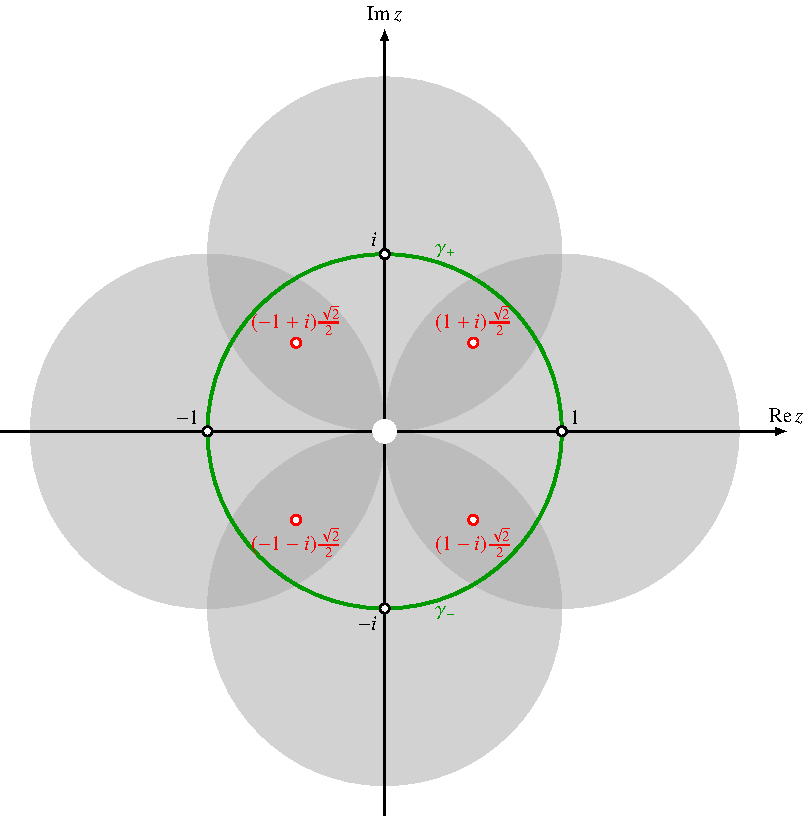
\includegraphics{chapters/080-funktionentheorie/images/fortsetzreziprok.pdf}
\caption{Analytische Fortsetzung für die Funktion $\frac1z$
entlang der Pfade $\gamma_+$ und $\gamma_-$.
\label{komplex:logfortsetzung}}
\end{figure}
Wir konstruieren jetzt die analytische Forstsetzung entlang der Kurven
$\gamma_+$ und $\gamma_-$ wie in Abbildung~\ref{komplex:logfortsetzung}
dargestellt.
Um die Differenz $C(z_1)-C(z_0)$ zu bestimmen, Werten wir die Funktionen
$F(z,z_0)$ und $F(z,z_1)$ jeweils im rot eingezeichneten Punkt aus.
Die exakte Berechnung ist etwas mühsam, da es sich ja nur um ein Beispiel
handelt, können wir die Reihen auch numerisch ausrechnen, und so die
Differenzen bestimmen:
\begin{align*}
&\text{Startpunkt $z_0=1$:}& C(1)&=0             &       &       \\
&\text{entlang $\gamma_+$:}& C(i)&= i\frac{\pi}2 & C(-1) &=  i\pi\\
&\text{entlang $\gamma_-$:}&C(-i)&=-i\frac{\pi}2 & C(-1) &= -i\pi
\end{align*}
Wir stellen fest, dass die analytische Fortsetzung der Logarthmusfunktion
entlang der Kurve $\gamma_+$ die Potenzreihe
\[
\log_+(z)
=
i\pi +\sum_{k=1}^\infty \frac{(-1)^{k+1}}{k(-1)^k}(z+1)^k
=
i\pi
-
\sum_{k=1}^\infty \frac{(z+1)^k}{k}
\]
ergibt, während man entlang der  Kurve $\gamma_-$
\[
\log_-(z)
=
-i\pi +\sum_{k=1}^\infty \frac{(-1)^{k+1}}{k(-1)^k}(z+1)^k
=
-i\pi
-
\sum_{k=1}^\infty \frac{(z+1)^k}{k}
\]
findet.
Die beiden analytischen Fortsetzungen entlang der Kurven $\gamma_+$ und
$\gamma_-$ stimmen auf der negativen reellen Achse nicht überein,
sie unterscheiden sich um $2\pi i$:
\[
\log_+(z)-\log_-(z)=2\pi i.
\qedhere
\]
\end{beispiel}

Das Beispiel zeigt, dass es im Allgmeinen eine auf der ganzen komplexen
Ebene definierte komplexe Entsprechung einer reellen Funktion nicht
zu geben braucht.
Dieses Phänomen tritt zum Beispiel auch bei der Wurzelfunktion $f(z)=\sqrt{z}$
auf.
Diese Funktion ist im Punkt $z=0$ nicht differenzierbar, man muss diesen
Punkt also aus dem Definitionsbereich ausschliessen.
Führt man man analog zum Beispiel eine analytische Fortsetzung durch,
findet man, dass sich die Werte von $f(z)$ für die beiden Wege $\gamma_+$
und $\gamma_-$ durch das Vorzeichen unterscheiden.
\subsection{Analytische Fortsetzung mit Differentialgleichungen
\label{komplex:analytische-fortsetzung-dgl}}
In Abschnitt~\ref{subsection:wegintegrale} wurde gezeigt, wie Wegintegrale
Stammfunktionen komplexer Funktionen liefern können.
Im vorangegangenen Abschnitt wurde untersucht, wie eine komplex differenzierbare
Funktion mit Hilfe von analytischer Fortsetzung entlang einer Kurve
ausgedehnt werden kann.

Sei $f(z)$ eine komplex differenzierbare Funktion.
In jedem beliebigen Punkt des Definitionsbereichs können wir $f(z)$
in eine Potenzreihe entwickeln, und natürlich auch termweise integrieren.
Es gibt also in jedem Punkt $z_0$ des Definitionsbereichs eine
Funktion $F_{z_0}(z)$, die $F'_{z_0}(z)=f(z)$ erfüllt.
Durch analytische Fortsetzung entlang einer Kurve $\gamma$ können
wir eine komplex differenzierbare Funktion $f(z)$ finden, die in einer
Umgebung der Kurve $F'(z)=f(z)$ erfüllt.

Sei andererseits $\gamma\colon[a,b]\to\mathbb C$ eine Kurve in $\mathbb C$.
Dann können wir die Werte der Stammfunktion im Punkt $\gamma(b)$ durch
\[
F(\gamma(b)) = F(\gamma(a))+\int_\gamma f(z)\,dz
\]
berechnen.

\begin{beispiel}
\begin{figure}
\centering
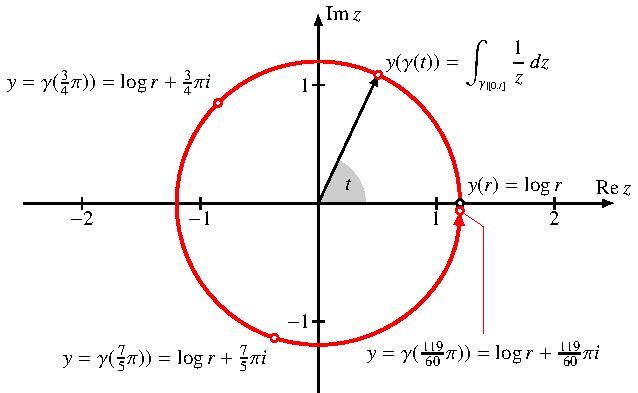
\includegraphics{chapters/080-funktionentheorie/images/logforts.pdf}
\caption{Analytische Fortsetzung des Logarithmus als Lösung der
Differentialgleichung $y'=\frac1z$.
Bei einem Umlauf um den Nullpunkt nimmt der Wert von $y(z)$ um
$2\pi i$ zu.
\label{komplex:analytische-fortsetzung-log}
}
\end{figure}
Wir bestimmen die Stammfunktion von $f(z)=1/z$.
Entlang der reellen Achse weiss man bereits, dass die Stammfunktion
der natürliche Logarithmus ist, also $F(x)=\log x$.
Um diese Stammfunktion auf $\mathbb C$ auszudehnen, verwenden wir einen
kreisförmigen Pfad von der reellen Achse bis zum Punkt $z$.
Liegt $z$ in der oberen Halbebene, wählen wir einen Pfad in der
oberen Halbebene, und umgekehrt.
Wir können die Zahl $z$ in Polarkoordinaten darstellen als $z=re^{i\varphi}$.
Ein Pfad von der reellen Achse kann mit
\[
\gamma\colon [0,1]\to\mathbb C: t\mapsto re^{it\varphi}
\]
parametrisiert werden.
Der Zuwachs der Stammfunktion entlang dieses Pfades ist
\[
F(z)-F(r)
=
\int_\gamma\frac1z\,dz
=
\int_0^1 \frac1{e^{it\varphi}}i\varphi e^{it\varphi}\,dt
=
i\varphi \int_0^1\,dt
=
i\varphi.
\]
Der Wert der Stammfunktion am Anfang der Kurve ist $\log r$, somit
folgt, dass
\[
\log z = \log r + i\varphi
\]
(Abbildung~\ref{komplex:analytische-fortsetzung-log}).
\end{beispiel}



%
% anwendungen.tex
%
% (c) 2021 Prof Dr Andreas Müller, OST Ostschweizer Fachhochschule
%
\section{Anwendungen
\label{buch:funktionentheorie:section:anwendungen}}

%
% gammareflektion.tex
%
% (c) 2021 Prof Dr Andreas Müller, OST Ostschweizer Fachhochschule
%
\subsection{Reflektionsformel für die Gamma-Funktion
\label{buch:funktionentheorie:subsection:gammareflektion}}
Die Formel~\eqref{buch:rekursion:gamma:spiegelung-betaintegral}
stellt eine Beziehung zwischen dem Produkt $\Gamma(x)\Gamma(1-x)$
von zwei Werten der Gamma-Funktion in Punkten der komplexen Ebene,
die durch Spiegelung an der Geraden $\operatorname{Re}x=\frac12$
auseinander hervorgehen, und einem speziellen Beta-Integral her.

\begin{satz}
\index{Satz!Spiegelungsformel für $\Gamma(x)$}%
\label{buch:funktionentheorie:satz:spiegelungsformel}
Für $0<x<1$ gilt
\begin{equation}
\Gamma(x)\Gamma(1-x)
=
\frac{\pi}{\sin\pi x}.
\end{equation}
\index{Gamma-Funktion!Spiegelungsformel}%
\end{satz}

\begin{figure}
\centering
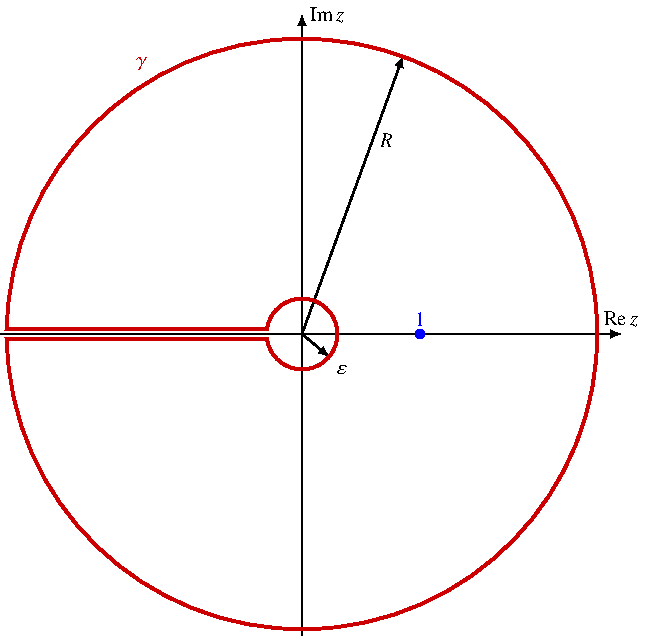
\includegraphics{chapters/080-funktionentheorie/images/gammapfad.pdf}
\caption{Pfad zur Auswertung des
Integrals~\eqref{buch:funktionentheorie:eqn:gammapfadintegral}
mit Hilfe des Residuensatzes.
\label{buch:funktionentheorie:fig:gammapfad}}
\end{figure}

\begin{proof}[Beweis]
In der Formel~\eqref{buch:rekursion:gamma:spiegelung-betaintegral}
wurde bereits ein Zusammenhang zwischen $\Gamma(x)\Gamma(1-x)$
und einem Beta-Integral hergestellt, konkret
\[
\Gamma(x)\Gamma(1-x)
=
B(x,1-x)
=
\int_0^1 t^{x-1}(1-t)^{-x}\,dt.
\]
Mit der Substitution $t=s/(s+1)$, die bereits für die Herleitung der
Formel~\eqref{buch:rekursion:gamma:beta:sinf} verwendet wurde, ergibt sich
\[
\Gamma(x)\Gamma(1-x)
=
\int_0^\infty 
\frac{s^{x-1}}{s+1}
\,ds.
\]
Um dieses Integral zu berechnen, verwenden wir den Cauchy-Integralsatz,
um das Integral
\begin{equation}
I
=
\oint_\gamma \frac{z^{x-1}}{1-z}\,dz
\label{buch:funktionentheorie:eqn:gammapfadintegral}
\end{equation}
zu berechnen.
Darin hat die Funktion im Zähler des Integranden $f(z)=z^{x-1}$ 
nur ausserhalb der negativen reellen Achse einen wohldefinierten Wert.
In Polarkoordinaten $z=re^{i\varphi}$ verwenden wir
den Hauptwert $z^{x-1}=r^{x-1}e^{i(x-1)\varphi}$.
Aus dem Cauchy-Integralsatz lesen wir den Wert
\[
I = 2\pi i
\]
ab.

Das Integral \eqref{buch:funktionentheorie:eqn:gammapfadintegral}
kann zerlegt werden in die Integrale
\begin{align*}
I
&=
I_R+I_++I_\varepsilon+I_-,
\end{align*}
wobei $I_R$ das Integral über den äusseren Kreis vom Radius $R$ ist,
$I_\varepsilon$ das Integral im Gegenuhrzeigersinn über den inneren Kreis
vom Radius $\varepsilon$.
Die Terme $I_{\pm}$ sind die Integrale entlang der negativen
reellen Achse, wobei das Pluszeichen für den oberen $-R$ nach
$-\varepsilon$ gelten soll.

Für die beiden Integrale $I_R$ und $I_\varepsilon$ wird die Parametrisierung
$\varphi\mapsto z(\varphi) = re^{i\varphi}$ mit $dz=ire^{i\varphi}\,d\varphi$
verwendet.
Das Integral über den Kreis vom Radius $r$ im Gegenuhrzeigersinn ist
\begin{align*}
I_r
&=
\int_{-\pi}^\pi
\frac{r^{x-1}e^{i(x-1)\varphi}}{1-re^{i\varphi}} ire^{i\varphi}\,d\varphi
=
i\int_{-\pi}^\pi
\frac{r^xe^{ix\varphi}}{1-re^{i\varphi}}
\,d\varphi
\end{align*}
Die beiden Teile $I_R$ und $I_\varepsilon$ können wie folgt noch
weiter vereinfacht werden:
\begin{align*}
\\
I_R
&=
iR^{x-1}
\int_{-\pi}^\pi
\frac{e^{ix\varphi}}{1/R-e^{i\varphi}}
\,d\varphi
\\
I_{\varepsilon}
&=
-
i
\varepsilon^x
\int_{\pi}^{-\pi}
\frac{e^{ix\varphi}}{1-\varepsilon e^{i\varphi}}
\,d\varphi,
\end{align*}
wobei das negative Zeichen bei $I_\varepsilon$ daher rührt, dass der
kleine Kreis im Uhrzeigersinn durchlaufen wird.
Für grosse Werte von $R$ ist das erste Integral beschränkt, aber wegen
$x-1<0$ konvergiert der Vorfaktor $R^{x-1}$ gegen 0 für $R\to\infty$.
Ähnlich ist das zweite Integral für kleine $\varepsilon$ beschränkt, aber
$\varepsilon^x$ konvergiert gegen $0$ für  $\varepsilon\to 0$.
Wir können daher
\begin{align*}
\lim_{R\to\infty}
I_R
&=
\lim_{R\to\infty}
R^{x-1}
\int_{-\pi}^\pi
\frac{e^{i(x-1)\varphi}}{1/R-e^{i\varphi}}
ie^{i\varphi}
\,d\varphi
=0
\\
\text{und}
\qquad
\lim_{\varepsilon\to 0}
I_\varepsilon
&=
-
\lim_{\varepsilon\to 0}
\int_{\pi}^{-\pi}
\frac{\varepsilon^{x-1}e^{i(x-1)\varphi}}{1-\varepsilon e^{i\varphi}}
i\varepsilon e^{i\varphi}
\,d\varphi
=
0
\end{align*}
folgern.

Die anderen zwei Integrale verwenden die Parametrisierung
$z(s) = -s = se^{\pm i\pi}$ mit $dz = e^{\pm i\pi}\,ds$.
Damit werden sie
\begin{align*}
I_+
&=
\int_{R}^{\varepsilon}
\frac{s^{x-1}e^{i(x-1)\pi}}{1-se^{i\pi}}
e^{i\pi}
\,ds
=
\int_{\varepsilon}^R
\frac{s^{x-1}e^{ix\pi}}{1+s}
\,ds
\\
I_-
&=
\int_{\varepsilon}^{R}
\frac{s^{x-1}e^{i(x-1)(-\pi)}}{1-se^{-i\pi}}
e^{-i\pi}
\,ds
=
-
\int_{\varepsilon}^{R}
\frac{s^{x-1}e^{-ix\pi}}{1+s}
\,ds.
\intertext{Die beiden Integrale stimmen bis auf den von $t$ unabhängigen
Faktor $e^{\pm ix\pi}$ überein, sie können daher zusammegefasst werden zu}
I_++I_-
&=
(e^{ix\pi}-e^{-ix\pi})
\int_{\varepsilon}^{R}
\frac{s^{x-1}}{1+s}
\,ds
=
\frac{e^{ix\pi}-e^{-ix\pi}}{2i}
\cdot
2i \int_{\varepsilon}^{R}
\frac{s^{x-1}}{1+s}
\,ds
\\
&=
2i
\sin(\pi x)
\int_{\varepsilon}^R
\frac{s^{x-1}}{1+s}
\,ds.
\end{align*}
Durch Grenzübergang $R\to\infty$ und $\varepsilon \to 0$ wird dies zu
\[
I
=
2i\sin(\pi x) \int_{0}^\infty \frac{s^{x-1}}{1+s}\,ds
\]
Zusammen mit dem früher bestimmten Wert $I=2\pi i$ folgt 
\[
2\pi i
= 
2i\sin(\pi x)
\int_{0}^\infty \frac{s^{x-1}}{1+s}\,ds
\qquad\Rightarrow\qquad
\frac{\pi}{\sin \pi x}
=
\int_{0}^\infty \frac{s^{x-1}}{1+s}\,ds
=
\Gamma(x)\Gamma(1-x).
\]
Damit ist der Satz bewiesen.
\end{proof}




\section*{Übungsaufgaben}
\rhead{Übungsaufgaben}
\aufgabetoplevel{chapters/080-funktionentheorie/uebungsaufgaben}
\begin{uebungsaufgaben}
%\uebungsaufgabe{0}
\uebungsaufgabe{1}
\uebungsaufgabe{2}
\end{uebungsaufgaben}

